\chapter{Digital Signal Processing Model} % Main chapter title

\label{ch_dsp_model} 

% Model Block Diagram -------------------------------------------------
\section{Model Block Diagram}
The blade imbalance detection is simulated using MATLAB/Simulink.  Figure \ref{fig:LIA_block_diagram} shows the block diagram for a method of imbalance detection where the rotor frequency is known.  This is an accurate method, but requires the information from an encoder on the shaft or an accurate phase-locked loop (PLL) controller.  

The force due to an imbalance is given in Equation \ref{eq:initial_force}.  It is a periodic function with the same frequency as the rotor and is proportional to the effective imbalance mass, $m$.  The variable forcing function is the input for the lumped parameter turbine tower state space model. These vibrations are then read by an acceleration sensor with a sampling rate of 100 Hz.  The frequency of interest is demodulated using a lock-in amplifier or DFT, which should result in the acceleration from only the imbalance.  The acceleration at the top of the tower should have higher amplitude vibrations at the rotor frequency when there is an imbalance in the blades (causing an eccentric mass).

\begin{figure}
	\centering
	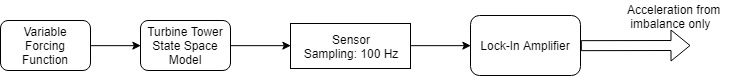
\includegraphics[scale=0.6]{LIA_block_diagram}
	\decoRule
	\caption{A block diagram showing the lock-in amplifier and the turbine tower simulation.  This figure was created with Draw.io.}
	\label{fig:LIA_block_diagram}
\end{figure}

%----------------------------------------------------------------------------------------

\section{Processing the data}

This paper describes a few ways to process the acceleration data from the turbine tower.  One method relies on accurate frequency information to precisely demodulate the signal at the rotor frequency.  An alternative method is to lock onto the strong frequency vibration of the tower using a phased-lock loop controller.  Finally, a discrete Fourier transform can be calculated to transform the time domain data to the frequency domain.  There are various ways to make this process more efficient, including zoom FFTs and the Goertzel algorithm.

The simulation and turbine tower state space model produce displacements shown in Figure \ref{fig:simulated_sensor_reading}.  The same simulation data is shown in the frequency domain  in Figure \ref{fig:sim_FFT_200RPM}.  From the frequency domain, it can be seen that there is resonance at 0.84 Hz (the natural frequency of the tower in the $x$-direction).  Additionally, there is an excitation at the rotor frequency that has a magnitude proportional to the amount of mass at the end of the blade.  This simplified linear model produces an displacement signal that can be represented by the sum of sines as shown in Equation \ref{eq:sum_of_sines} (this can be seen in Figure \ref{fig:simulated_sensor_reading}).
\begin{equation} \label{eq:sum_of_sines}
	y = C_1 \sin{(\omega_n t + \phi_1)} + C_2 \sin{(\omega_{drive} t + \phi_2)}
\end{equation}

The first method for processing the acceleration data utilizes a lock-in amplifier to translate the data in the frequency domain.  This new data, with the rotor frequency shifted to 0 Hz, is filtered and results in a DC acceleration that should be proportional to the imbalance mass.  The second method utilizes a zoom FFT, which provides higher resolution than a typical FFT in the bandwidth of interest.  The third method uses a Goertzel algorithm to calculate the bin of interest in the DFT.

\begin{figure}
	\centering
	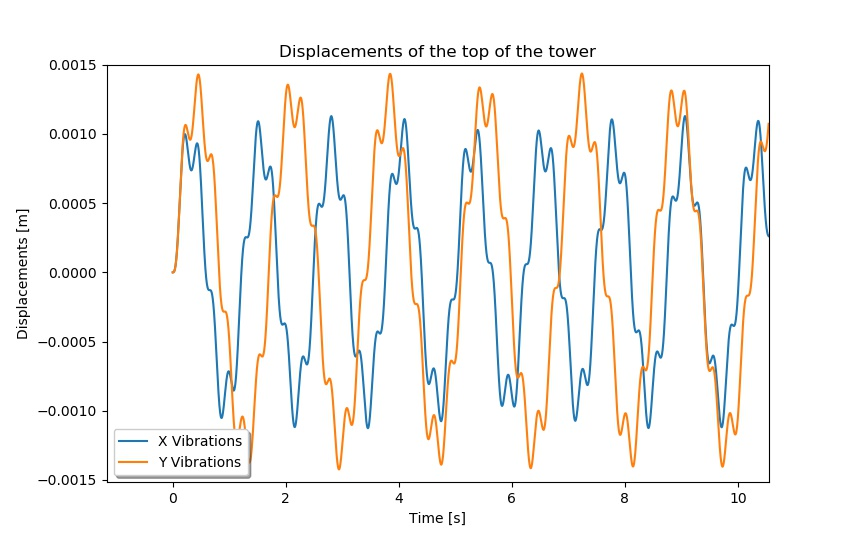
\includegraphics[scale=0.6]{simulated_sensor_reading}
	\decoRule
	\caption{The simulated displacement for a rotor imbalance at 230 RPM.  The imbalance mass is placed at the end of the blade, which causes accelerations and displacements at the top of the tower.  This figure was created with Python.}
	\label{fig:simulated_sensor_reading}
\end{figure}

\begin{figure}
	\centering
	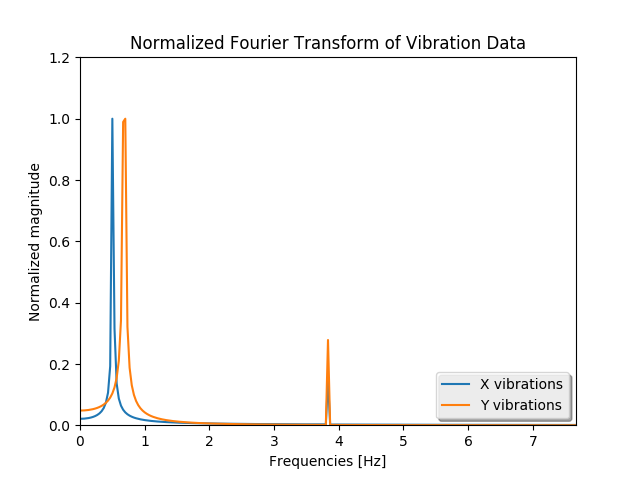
\includegraphics[scale=0.6]{sim_FFT_200RPM}
	\decoRule
	\caption{This figure shows the simulated displacement data in the frequency domain.  The rotor frequency is 230 RPM in this simulation. This figure was created with Python.}
	\label{fig:sim_FFT_200RPM}
\end{figure}

\subsection{DFT review}
A Discrete Fourier Transform (DFT) converts a signal from the time domain to the frequency domain.  Typically, this is performed with using the Fast Fourier Transform (FFT) algorithm, which is an efficient method for calculating the DFT.  The DFT is defined by the formula in Equation \ref{eq:dft_definition} \cite{winograd1976computing}.
\begin{equation} \label{eq:dft_definition}
	X_k = \sum_{n=0}^{N-1}{x_n \cdot e^{-\frac{i 2 \pi}{N} k n}}
\end{equation}

$\vec{x}$ is the original signal in the time domain with $N$ elements, and $\vec{X}$ is the signal in the frequency domain with $N$ elements.  Equation \ref{eq:dft_definition} can be rewritten using Euler's formula to show DFT equation in terms of sine and cosine values (this is important for understanding the lock-in amplifier in a future section).  Equation \ref{eq:dft_euler} shows the new expression for the DFT equation.
\begin{equation} \label{eq:dft_euler}
	X_k = \sum_{n=0}^{N-1}{x_n \cdot \left[ \cos{\left(\frac{2 \pi k n}{N}\right)} - j \sin{\left(\frac{2 \pi k n}{N}\right)} \right]}
\end{equation}

From Equation \ref{eq:dft_euler}, it can be seen that the DFT can be calculated by mixing the signal, $\vec{x}$, with a sine and cosine signal and summing the result for each frequency.  The DFT equation can be further rewritten using vector notation as in Equation \ref{eq:dft_vector} and defining some reference vectors.  This equation shows that the DFT of a signal is an imaginary vector that can be created from the dot products of the original signal and some reference sine and cosine signals.
\begin{align}
	\vec{n}_r &= 
		\begin{bmatrix}
			0/N \\
			1/N \\
			2/N \\
			\vdots \\
			(N-1)/N	
		 \end{bmatrix} \\
	\vec{r}_{sin} &= \sin{\left(2 \pi k \vec{n}_r\right)} \\
	\vec{r}_{cos} &= \cos{\left(2 \pi k \vec{n}_r\right)} \\
	X_k &= \vec{x}^T \cdot \vec{r}_{cos} - j \vec{x}^T \cdot \vec{r}_{sin}  \label{eq:dft_vector}
\end{align}

Another way of looking at the DFT (from the form in Equation \ref{eq:dft_vector}) is as a time domain convolution with a low pass filter.  The summation (shown explicitly in the form from Equation \ref{eq:dft_euler}) acts as a simple finite impulse response (FIR) decimation filter with unity coefficients and a decimation rate of $d=N$, commonly known as an averaging filter.  When thinking about the DFT in this way, some possible optimization methods start to become clear.  For example, we may not need to calculate the frequency component for every $k$th element in $\vec{X}$, and we may choose to use a better filter that has stronger attenuation at higher frequencies.  This is the basis for the lock-in amplifier design described in the next section.


\subsection{Lock-In Amplifier}

A lock-in amplifier is used to measure AC signals in particularly noisy environments (Figure \ref{fig:LIA}).  It works by multiplying the noisy signal by a reference signal created by an internal oscillator.  By using two reference signals out of phase, the real and imaginary parts of the signal at the specified carrier frequency can be calculated \cite{LIA_applications}.  Let's say there is an unknown sinusoidal signal with high frequency noise ($\omega_2 >> \omega_1$):
\begin{equation}
	y = A \,\sin{(\omega_1 \, t)} + B\,\sin{(\omega_2 \, t)}
\end{equation}

The amplitude of the signal, $A$, can be determined by multiplying the signal, $y$, by a reference signal with the same frequency as $\omega_1$ and filtering:
\begin{align}
	y \cdot \sin{(\omega_1 \, t)} &= \, \left[A \,\sin{(\omega_1 \, t)} + B\,\sin{(\omega_2 \, t)}\right] \, \sin{(\omega_1\,t)} \label{eq:sine_LIA}\\
	&=A\,\sin^2{(\omega_1\,t)} + B\,\sin{(\omega_1\,t)}\,\sin{(\omega_2\,t)} \\
	&=A\left(\frac{1}{2} - \frac{1}{2}\,\cos{(2\,\omega_1\,t)}\right) + B\,\sin{(\omega_1\,t)}\,\sin{(\omega_2\,t)} \label{eq:LIA_equation}
\end{align}

Note that Equation \ref{eq:sine_LIA} resembles the imaginary part of the standard DFT equation (Equation \ref{eq:dft_euler}), where the input signal is multiplied by a sine wave at a set reference frequency.

A filter is applied to Equation \ref{eq:LIA_equation} (similar to the summation filter used in Equation \ref{eq:dft_euler}), with a cutoff frequency that is smaller than $\omega_1$.  This results in all terms approaching zero, except for $\frac{A}{2}$, which can be calculated and solved for $A$ to achieve the magnitude of the frequency component at $\omega_1$.  To calculate the magnitude and phase of the signal $y$, it must be multiplied by a reference sine signal (as in Equation \ref{eq:sine_LIA}) and a reference cosine signal.  The following equation shows the result of the mixing step (phase-sensitive detection) in the lock-in amplifier:
\begin{equation} \label{eq:LIA_mixing}
	Y = X \cos{(\omega t)} + j X \sin{(\omega t)}
\end{equation}

where $X$ is the noisy AC signal and $Y$ is the signal that is fed into a filter to remove any unwanted frequency components at $\omega_1$ and $2 \omega_1$ and produce a signal, $Y_{filtered}$ that only contains the DC component:
\begin{equation}
	Y_{filtered} = \frac{A_{real}}{2} + j \frac{A_{imaginary}}{2}
\end{equation}

\begin{figure}
	\centering
	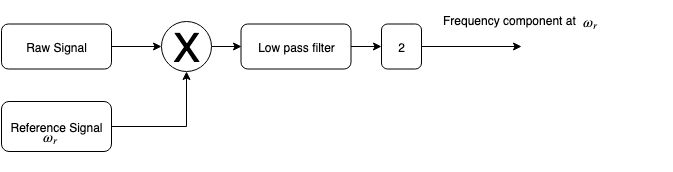
\includegraphics[scale=0.7]{LIA}
	\decoRule
	\caption{A block diagram showing the details of a lock-in amplifier.  This figure was created with Draw.io.}
	\label{fig:LIA}
\end{figure}

Using the lock in amplifier tuned to a constant frequency, Figure \ref{fig:200_RPM_LIA_output_sim} shows the resulting output.  This shows that an imbalance can be detected by measuring the output of a lock-in amplifier that is tuned to the frequency of the turbine rotor.  When the acceleration data is treated as an AM signal, with the carrier frequency equal to the rotor frequency, the acceleration due to the rotation of the blades can be identified.  This acceleration is directly related to the mass at the end of the blade, and should be a constant value (as long as the rotor frequency is accurately known).

Lock-in amplifiers (LIAs) are typically used when the frequency is relatively stable and the signal-to-noise ratio is low.  For this application, the rotor frequency can change, which may not give the LIA filters enough time to settle.  If there is a very stable and accurate rotor speed controller, this method would be ideal because it extracts the signal of interest despite the high noise and distortions in the measurement.

\begin{figure}
	\centering
	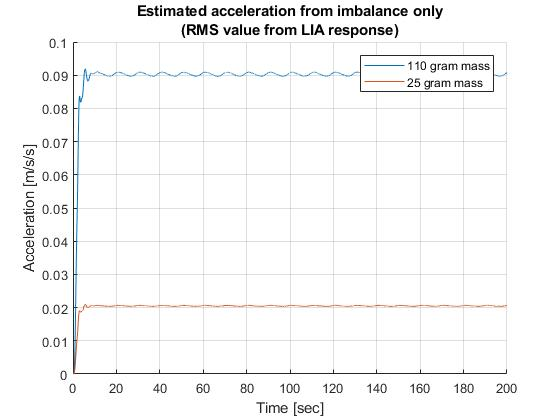
\includegraphics[scale=0.7]{200_RPM_LIA_output_sim}
	\decoRule
	\caption{The output of the lock-in amplifier from the simulated data shown in Figure \ref{fig:simulated_sensor_reading}.  This figure was created with Python.}
	\label{fig:200_RPM_LIA_output_sim}
\end{figure}


\subsubsection{Types of low-pass filters}
The filter choice is very important for a lock-in amplifier.  Some of the common options are finite impulse response (FIR) filters, and infinite impulse response (IIR) filters, and the Savitzky-Golay (SG) filter.

The IIR filter is shown in Figure \ref{fig:IIR_block_diagram}, which significantly smooths the data, but at the cost of some time-domain distortion.  An IIR filter uses past states in the output calculation, meaning an impulse input signal will affect the filter output forever (\textit{infinite} impulse response filter).  This results in a transfer function as follows:

\begin{equation} \label{eq:IIR_tf}
	T(z) = \frac{b(z)}{a(z)}
\end{equation}

\begin{figure}
	\centering
	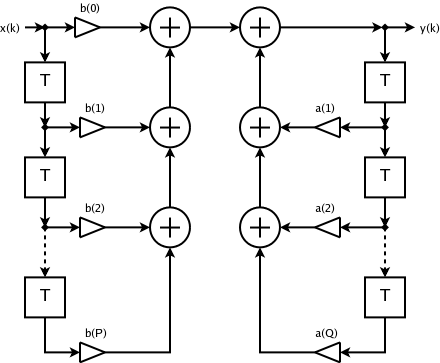
\includegraphics[scale=0.5]{IIR_block_diagram}
	\decoRule
	\caption{A block diagram of a standard IIR filter. \cite{wiki:IIR_block_diagram}}
	\label{fig:IIR_block_diagram}
\end{figure}


Figure \ref{fig:IIR_filter_response} shows the result of a Butterworth IIR filter compared to a moving average filter.  This shows that a customized filter is much more effective than standard moving average methods of smoothing data.

\begin{figure}
	\centering
	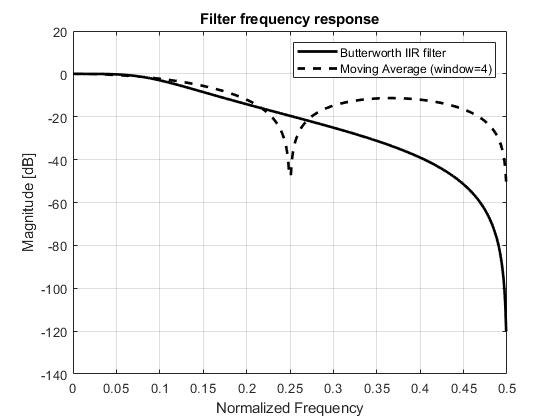
\includegraphics[scale=0.8]{IIR_filter_response}
	\decoRule
	\caption{The filter response of the Butterworth IIR filter (Equation \ref{eq:IIR_tf}) compared to a moving average filter with a window size of 4.  This figure was created in MATLAB with 2 simulated filter designs.}
	\label{fig:IIR_filter_response}
\end{figure}


Another filter alternative is the FIR filter, which does not rely on past states to calculate the filter output.  This results in a finite response to an impulse input and a linear phase.  A common FIR filter that is used for smoothing data is a moving average (where all of the filter coefficients are identical).  To achieve a more customized filter for this data, a FIR filter is designed using the Window method, which designs a FIR filter using a specified window.  Figure \ref{fig:FIR_block_diagram} shows a block diagram of a FIR filter.  One of the most common uses of FIR filters is to decimate a signal (not having to calculate previous states allows for some significant optimizations when decimation is involved).  Because the past states are not used, the transfer function has a denominator of 1:

\begin{equation}
	T(z) = \frac{b(z)}{1}
\end{equation}

\begin{figure}
	\centering
	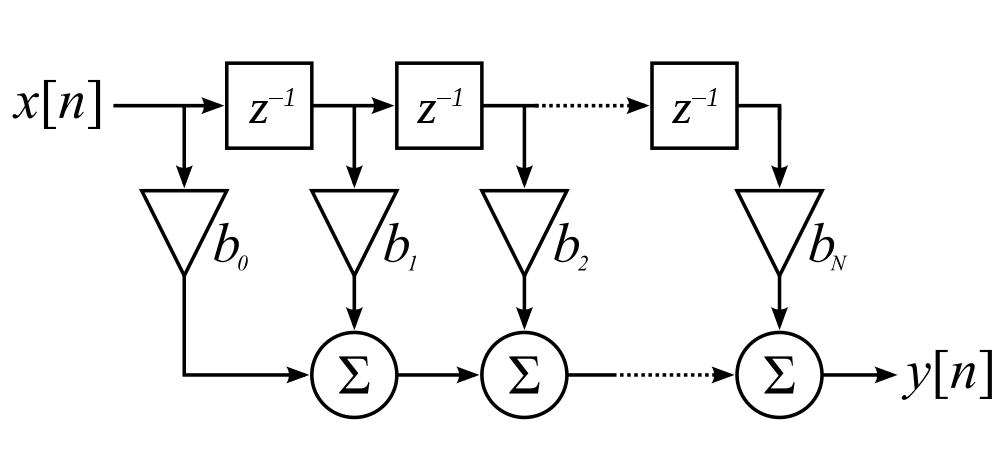
\includegraphics[scale=0.3]{FIR_block_diagram}
	\decoRule
	\caption{A block diagram of a standard FIR filter. \cite{wiki:FIR_block_diagram}}
	\label{fig:FIR_block_diagram}
\end{figure}

Another filter option for this data is the Savitzky-Golay (SG) filter, which increases the signal-to-noise ratio with out significantly distorting the signal.  The SG filter uses convolution to fit a polynomial on a sliding window to the data.  The output of this filter can be calculated using the following equation \cite{SG_filter}:

\begin{equation} \label{eq:SG_filter}
	Y_j = (\mat{C} \otimes y)_j = \sum_{i=-\frac{m-1}{2}}^{\frac{m-1}{2}} C_iy_{j+i}
\end{equation}

$C_i$ are the convolution coefficients ($m$ total coefficients), $y$ is the sampled data point, and $j$ is the index of the data point. 

The convolution coefficients can be selected from a table, but it is much more robust to calculate them prior to performing any filtering.  The convolution coefficients, $\mat{C}$, are calculated using a variable change.  The time vector for a given window, $\vec{x}$, is converted to $\vec{z}$ using the time step ($\Delta t$) with the following equation:

\begin{equation}
	z = \frac{\vec{x} - \bar{x}}{\Delta t}
\end{equation}

$\bar{x}$ is the time value at the central point of the window.  $\vec{z}$ is used to calculate the matrix $\mat{J}$, where each $i\mathrm{-th}$row of $\mat{J}$ has the values $1, z_i, z_i^2, z_i^3, ..., z_i^n$.  After $\mat{J}$ has been created, the convolution coefficients can be calculated as follows:

\begin{equation}
	\mat{C} = \left(\mat{J^TJ}\right)^{-1}\mat{J^T}
\end{equation}

The filtered data can then be calculated as the convolution of $\mat{C}$ and the unfiltered data (Equation \ref{eq:SG_filter}).



\subsection{Identifying the rotor frequency from the tower accelerations}
If the rotor frequency cannot be measured directly, it is possible to obtain the frequency indirectly from the acceleration data.  A phase-locked loop is a control system that minimizes the phase between to signals.  As the phase error is driven to zero, the output signal frequency approaches the input signal's frequency.  Phase-locked loops (PLLs) are commonly used in telecommunications where the frequency of a noisy signal can be recreated with an internal oscillator that locks on to the frequency of the noisy signal.  Figure \ref{fig:PLL_diagram} shows a block diagram of the PLL implementation with tower acceleration data as the input.

The first stage of the frequency detection is a narrow bandpass filter to get rid of high frequency noise and natural frequency resonance of the tower.  This is multiplied by an internal oscillator that starts at an arbitrary frequency (a guess that is close to the actual frequency, but not necessarily accurate).  This signal is passed through a lowpass filter to provide a steady phase error.  The phase error is driven to 0 using a PID controller.  This outputs the correct frequency of the signal that is then fed back and multiplied with the input signal.

One of the problems with a phase-locked loop is that the PID controller gains depend on the amplitude of the signal, which changes depending on the amount of imbalance and rotor frequency.  The simplest approach to this would be to normalize the accelerations with the expected frequency.  This, however, is not perfect and doesn't account for the acceleration variation due to different eccentric masses.  A better solution would be to use a simple envelope detector to determine the amplitude of signal.  The accelerations can be divided by the output of the envelope detector to normalize the signal.  Figure \ref{fig:envelope_detector} shows an example of a simple envelope detector\cite{envelope_detector_ref}.  The low-pass filter in the envelope detector can be designed based on the desired accuracy.  For high computational efficiency, an averaging filter can be used because it minimizes the amount of multiply operations, and reduces the filter calculation to summations only.

\begin{figure}
	\centering
	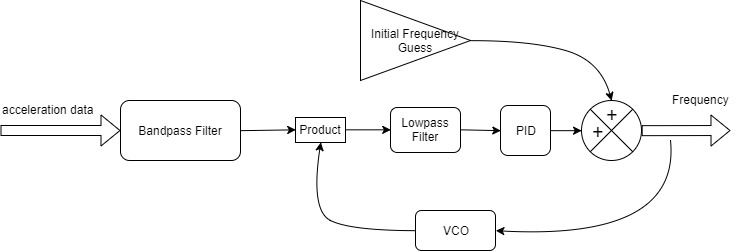
\includegraphics[scale=0.5]{PLL_diagram}
	\decoRule
	\caption{The block diagram of a phase-locked loop implementation when detecting rotor frequencies from acceleration measurements \cite{embedded_zoom_fft}.  This diagram was created with Draw.io \cite{draw_io}.}
	\label{fig:PLL_diagram}
\end{figure}

\begin{figure}
	\centering
	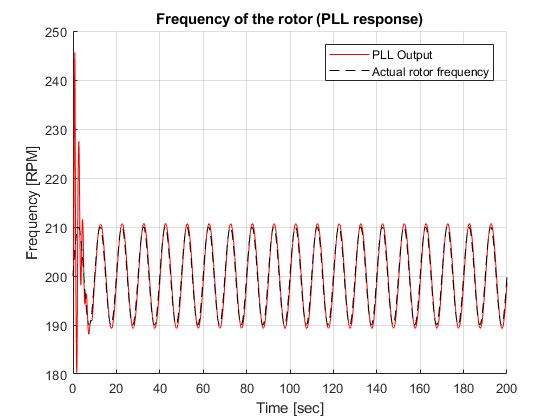
\includegraphics[scale=0.5]{PLL_simulation}
	\decoRule
	\caption{The output of the PLL  when detecting frequency from the data shown in Figure \ref{fig:simulated_sensor_reading}.  The frequency of the input data oscillates from 190 RPM to 210 RPM to simulate a real turbine controller that may oscillate between frequencies.  This figure was created with MATLAB.}
	\label{fig:PLL_simulation}
\end{figure}

\begin{figure}
	\centering
	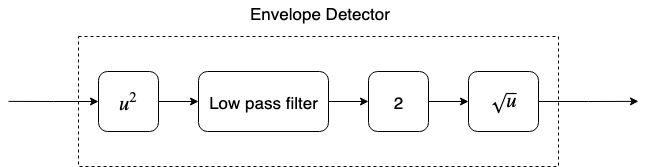
\includegraphics[scale=0.5]{envelope_detector}
	\decoRule
	\caption{A block diagram for a simple envelope detector.  The signal is first squared and multiplied by a gain of 2.  This signal (which should be entirely positive) is sent through a lowpass filter to remove the high frequency information.  The lowpass filter needs to reject $2f$, which is the resulting frequency when a signal with frequency, $f$ is squared.  The square root of the resulting signal produces the the amplitude of the signal.  This figure was created with Draw.io.}
	\label{fig:envelope_detector}
\end{figure}

\subsection{Windowed FFT}
One problem with standard FFTs is that the frequency content can get spread across all of the bins if the signal contains frequencies that do not fall exactly into any one bin.  For example, a 1024-point FFT of a signal sampled at 128 Hz will have bins at each integer frequency value (0,1,2,3, ..., 64 Hz).  If the measured signal contains a signal at 10.l Hz, the frequency spectrum will spread this component across all of the bins.  This is shown by the standard FFT in Figure \ref{fig:MATLAB_fft_window}.  In order to prevent this from happening, a windowing filter can be applied to the raw signal before the FFT is calculated.  These windowing filters are weighted averages of the signal (rather than a uniform average that is performed by the standard FFT).  Two of the most common windowing filters are the Blackman and Hamming windows.  For FFT analysis, the Blackman filter is preferable because it has a narrower peak and rejects some of the higher frequencies more than the Hamming window.  Figure \ref{fig:MATLAB_fft_window} shows the result of a standard FFT and a windowed FFT applied to the same signal.

To apply a windowed FFT, the coefficients ($\vec{w}$) of the Blackman (or other windowing function) function must be created.  The Blackman coefficients can be created analytically in Equation \ref{eq:blackman} \cite{MATLAB_blackman}.  In this equation, $N$ is the length of the windowing filter (which is equal to the number of points in the FFT).
\begin{equation} \label{eq:blackman}
	\vec{w}(n) = 0.42 - 0.5 \cos{\left(\frac{2 \pi n}{N-1}\right)} + 0.08 \cos{\left(\frac{4 \pi n}{N-1}\right)}, \,\,\,\,\, 0 \leq n \leq (N-1)
\end{equation}

The Blackman coefficients are then element-wise multiplied by the signal ($\vec{y}$) before the FFT is calculated as shown in Equation \ref{eq:apply_window_filter} ($\odot$ is the element-wise multiplication operator).
\begin{align}
	\vec{y}_{window} &= \vec{y} \odot \vec{w} \\
	m_{fft} &= \texttt{FFT}\left(\vec{y}_{window} \right) \label{eq:apply_window_filter}
\end{align}


\begin{figure}
	\centering
	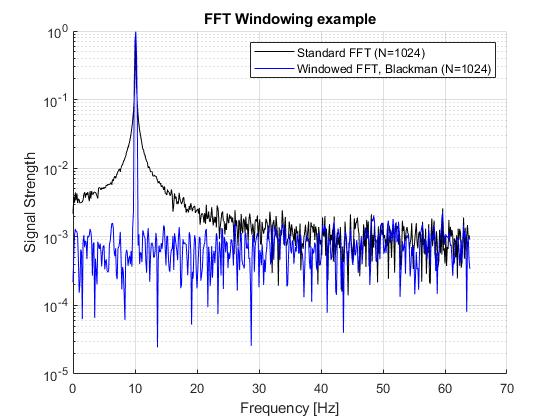
\includegraphics[scale=0.7]{MATLAB_fft_window}
	\decoRule
	\caption{This figure shows a standard FFT and a windowed FFT with a sampling rate of 128 Hz.  The FFT length is 1024, and the windowing filter is a Blackman filter.  This figure was created with MATLAB.}
	\label{fig:MATLAB_fft_window}
\end{figure}



\subsection{Zoom FFT}
A very powerful method for reducing the computational cost of the FFT calculation is to use a Zoom FFT.  If the imbalance detection device contains a low-power processor, it will be able to run for a long time off of a battery.  This also means that the processor could be much slower than an alternative high-power processor.  A Zoom FFT will significantly reduce the computational load on the processor, allowing the low-power processor to sufficiently calculate the frequency spectrum of the input signal.

One of the main tradeoffs for the reduced computational load, is a reduced frequency spectrum range.  For example, a set of 1024 data points sampled at $F_s$, will produce a frequency spectrum from $0$ to $F_s/2$ using the standard FFT.  A zoom FFT with a decimation rate of $D=10$ can produce a frequency spectrum with a range of $F_s/20$ at 1/10th the computational cost.

If the frequency of the rotor is not precisely known, then a lock-in amplifier is difficult to implement.  In order to detect excitation at the rotor frequency, the time-domain data can be transformed into the frequency domain.  A discrete Fourier transform (DFT) is the frequency domain representation of a sampled signal; however, it can be slow and difficult to calculate on a microcontroller.

To efficiently calculate the Fourier transform, the DFT matrix can be factored and the complexity reduced from $O(n^2)$ to $O(n \log{n})$.  This efficient algorithm is called the fast Fourier transform (FFT).  Despite being much more efficient than the standard DFT, a generic FFT is still inefficient for this application because most of the frequency data occurs outside the bandwidth of interest and is thrown away.  This can be fixed by applying a zoom FFT algorithm.

The zoom FFT consists of 4 main steps.  First the data is convoluted with a reference signal in the time domain (translated in the frequency domain) to shift a center frequency, $F_c$, to 0 Hz.  Second, a lowpass filter prevents aliasing when sampling at a lower sample rate.  An infinite impulse response (IIR) filter can be used for simplicity; however, the phase information of the signal is lost.  To solve this, a finite impulse response (FIR) filter can be used.  FIR filters are more complicated but most have a flat phase response, ensuring the filter output retains the original phase information.  Third, the data is decimated (re-sampled at a lower rate). Finally, the decimated data is passed through a FFT algorithm that produces a frequency spectrum in the specified bandwidth.  Since the frequency range of the zoom FFT is much smaller, the resolution can be much higher for a FFT length.  Alternatively, a much smaller FFT length can be used to produce the same resolution.

For a microcontroller sampling the acceleration of the turbine tower at 128 Hz, Figure \ref{fig:zoom_fft_diagram} shows a block diagram of a zoom FFT implementation for detecting an imbalance.  Point A represents the raw input signal, which is the acceleration of the tower sampled at $F_s=128$ Hz in this case.  The frequency translation is performed by mixing the input signal with a reference signal at $F_c$.  The goal of a Zoom FFT is to reduce the amount of data by decimating the original signal and reducing the sampling rate.  Just performing a sampling rate reduction would result in aliasing, so there needs to be a digital anti-aliasing filter that prepares the signal for the decimation step.  This digital filter is a low pass FIR filter that produces a filtered signal at Point C, which can then be decimated without aliasing to achieve Point D.  This new set of data is sampled at $F_{s,new}=\frac{F_s}{D}$, which means the frequency spectrum spans a much smaller range.

Zoom FFTs \cite{zoom_fft_ref} contain the following parameters:

$F_c$: The frequency center (shifted to 0 Hz by the zoom FFT) \\
$BW$: The bandwidth of interest \\
$F_s$: The sampling rate \\
$N$: The length of the FFT

The decimation factor, $D$, is calculated as follows:
$$D = floor\left(\frac{F_s}{BW}\right)$$

Where the length, $L$, of the initial buffer into the decimator is:
$$L=D \cdot N$$

\begin{figure}
	\centering
	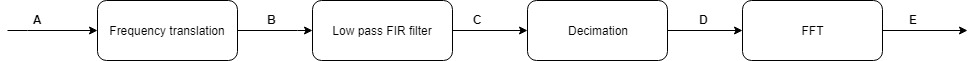
\includegraphics[scale=0.4]{zoom_fft_diagram}
	\decoRule
	\caption{A block diagram showing the zoom FFT algorithm. This figure was created with Draw.io.}
	\label{fig:zoom_fft_diagram}
\end{figure}

The computational reduction for a Zoom FFT is shown in Figure \ref{fig:zoom_fft_complexity_reduction}.  However, it is important to note that a stronger filter is required for higher decimation factors, $D$.  This means there is a trade-off between FFT computational load and filter computational load.  A zoom FFT is just the name of a method of frequency transformation where the data is decimated before applying the FFT algorithm.  The computational savings occur when a well-designed lowpass filter does not negate the workload reduction caused by the FFT.  Essentially, this is a much more flexible FFT where different aspects can be modified to optimize for the application.  In this case, the Zoom FFT can provide a much higher resolution frequency analysis because the frequencies of interest are much smaller than the sampling rate.


\begin{figure}
	\centering
	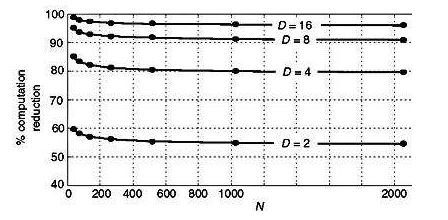
\includegraphics[scale=0.8]{zoom_fft_complexity_reduction}
	\decoRule
	\caption{A diagram showing the percent computational workload reduction of a $\frac{N}{D}$-point Zoom FFT relative to a standard $n$-points FFT \cite{embedded_zoom_fft}.}
	\label{fig:zoom_fft_complexity_reduction}
\end{figure}



\subsubsection{Frequency translation}
Shifting data in the frequency domain is a common technique used in AM radio signals.  Audio frequencies are typically mixed with a high frequency carrier that, according to the Nyquist criteria, would require an extremely high sample rate to capture the signal.

If $\omega$ is the rotor frequency, multiplying the time domain signal by $\cos{(-\omega t)}$ is the same as convolving the data in the frequency domain.  Since the frequency spectra for $\cos{(-\omega t)}$ is symmetric across the y-axis, the time-domain must be multiplied by an imaginary wave.

The equation for the frequency-shifted time-domain data is:
\begin{equation} \label{eq:frequency_translation}
	Y = X e^{-i (\omega t)}
\end{equation}

where $Y$ is the shifted data, $X$ is the original data, $\omega$ is the rotor frequency, and $t$ is the time.  Based on Equation \ref{eq:frequency_translation}, the real and imaginary parts of the shifted signal are shown below \cite{zoom_fft_ref}:
\begin{align}
	Y_{real} = X \cos{(\omega t)} \\
	Y_{imaginary} = -X \sin{(\omega t)} \label{eq:freq_trans_im}
\end{align}

An example of frequency translation is shown in Figure \ref{fig:MATLAB_freq_translation_ex}.  The blue signal is the frequency-shifted signal, which has a higher frequency at 2 times the original signal frequency.  In order to remove the extra component at 10 Hz, the digital filter (shown with a dotted blue line) must be applied to the shifted signal.

\begin{figure}
	\centering
	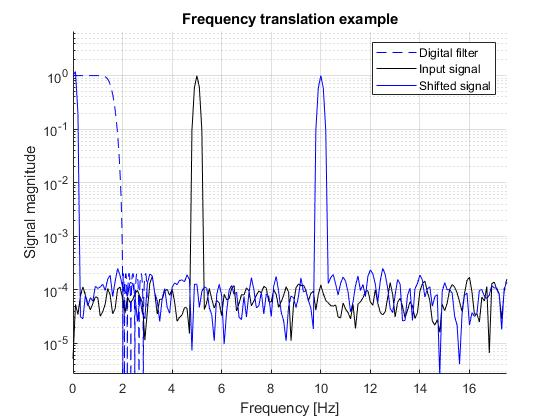
\includegraphics[scale=0.7]{MATLAB_freq_translation_ex}
	\decoRule
	\caption{This figure shows an example of frequency translation.  The black signal is the frequency spectrum of some input signal that has a strong component at 5 Hz.  The blue signal shows the frequency shifted spectrum that results from multiplying the input signal by a reference signal with a frequency of 5 Hz (as shown in Equation \ref{eq:freq_trans_im}).  The dotted blue line shows the digital filter response.  This figure was generated with MATLAB.}
	\label{fig:MATLAB_freq_translation_ex}
\end{figure}

\subsubsection{Decimation/downsampling}
Decimation is the process of reducing the sample rate of a signal.  Before the data is downsampled, the high frequency components are reduced with a lowpass filter. This filter is also called an anti-aliasing filter because it prevents high frequency data from being misinterpreted at a different sample rate.  Equation \ref{eq:decimation} shows the equation used for calculating the output of a FIR decimator, where $x$ is the input data, $h$ is the impulse response, $K$ is the length, and $D$ is the decimation factor\cite{decimation_ref}.
\begin{equation} \label{eq:decimation}
	y[n] = \sum_{k=0}^{K-1} x[nD-k] \cdot h[k]
\end{equation}

Figure \ref{fig:MATLAB_freq_translation_ex} shows a visual representation of the decimation process and anti-aliasing filter.  The shifted signal (blue) contains important frequency information in the range 0 - 2 Hz.  Any higher frequencies have been significantly attenuated by the digital filter (dotted blue line).  This means the blue data can be decimated to a new sampling rate of 4 Hz, without any aliasing effects (because the digital filter ensures there are no strong components above 2 Hz).



\subsubsection{An optimized Zoom FFT implementation}

Table \ref{t:zoom_fft_parameters} shows the parameters for the Zoom FFT.  These values have been strategically picked to make the optimization process easier.  In general, some nice optimizations can be achieved if the number of filter coefficients ($N_b+1$) is an integer multiple of the sampling rate ($F_s$).

\begin{table}[]
\centering
\caption{Zoom FFT parameters}
\label{t:zoom_fft_parameters}
\vspace*{0.2in}
\begin{tabular}{|c|c|c|}
\rowcolor[HTML]{EFEFEF} 
\hline
\textbf{Variable} & \textbf{Value} & \textbf{Description} \\ \hline
$F_{min}$ & 2 Hz & The minimum frequency for the Zoom FFT calculation\\ \hline
$F_s$ & 128 Hz & The original sampling rate\\ \hline
$F_r$ & 4 Hz & The frequency range of the Zoom FFT\\ \hline
$N_{fft}$ & 128 & FFT length (buffer length used in the FFT calculation)\\ \hline
$N_b$ & 255 & FIR filter order \\ \hline
$D$ & $\frac{F_s}{2 F_r}=16$ & Decimation rate \\ \hline
\end{tabular}
\end{table}

In Table \ref{t:zoom_fft_parameters}, the FFT length is the number of samples in the buffer used as the input to the FFT. An FFT length of 1024 means that 1024 samples are used as an input to the FFT algorithm.  The FIR filter order is 255, which is high because it needs to strongly attenuate higher frequencies with a narrow pass band.  Despite having an extremely large order, the FIR filter is simple and computationally inexpensive to implement (this will be shown later in this section).  An order of $N_b=255$ means the filter order will have 256 ($N_B+1$) coefficients.  $F_{min}$ and $F_r$ define the frequency range that the Zoom FFT is targeting.  More specifically, the Zoom FFT will calculate the frequency spectrum of the input signal only from $F_{min}$ to $F_{r}$.  The filter design is highly motivated by the frequency range because it needs to attenuate the original signal sufficiently (to prevent aliasing at the decimation step) at the edge of the frequency range.

The reference signal for the Zoom FFT is created at the minimum frequency, $F_{min}$ shown in Table \ref{t:zoom_fft_parameters} and is shown in Equation \ref{eq:zoom_ref_sig}.
\begin{equation} \label{eq:zoom_ref_sig}
	y_{ref} = \sin{(F_{min} \cdot 2\pi \cdot time)}
\end{equation}

Note that there are only 64 unique values in a reference signal with the specified $F_{min}$.  This means that all of these values can be precomputed at initialization and stored in memory.  This removes the $\sin{()}$ operations from the real-time calculations, which reduces the computational time, since trig functions are one of the slowest floating-point operations (they are typically about 15X slower than a floating-point addition operation) \cite{flops_performance}.

One of the benefits for using a finite impulse response (FIR) filter is that there are no recursive calculations.  This produces a very important property of FIR filters, which is that not all the outputs need to be calculated.  Assuming there are ($N_b+1$) filter coefficients, a random window of ($N_b+1$) samples can be properly filtered at any time during operation.  If we are decimating the input signal, this means we do not have to calculate the filter outputs for samples that are removed due to the decimation step.

The down-sampled data, $y_{ds}$, can be calculated as follows ($\odot$ is the element-wise multiplication operator):
\begin{equation} \label{eq:zoom_y_ds}
	y_{ds} = \vec{y}^T \cdot \left( \vec{y}_{ref} \odot 2\vec{b} \right)
\end{equation}

In Equation \ref{eq:zoom_y_ds},  $y_{ds}$ is the value at the decimated sampling rate.  $\vec{y}$ is a sliding buffer of the original input data, which is a vector of ($N_b+1$) values.  $\vec{y}_{ref}$ is the vector of the reference signal values, which also has a length of ($N_b+1$).  $\vec{b}$ is the vector of FIR filter coefficients.  The factor of 2 in this equation is a result of the derivation of the frequency-shift process.  Equation \ref{eq:zoom_y_ds} is calculated at the decimated sampling rate ($F_{sD}$), which is shown in Equation \ref{eq:zoom_dec_Fs}.
\begin{equation} \label{eq:zoom_dec_Fs}
	F_{sD} = \frac{F_s}{D}
\end{equation}

Equation \ref{eq:zoom_y_ds} can also be used with larger filter orders.  Effectively, this means that the filtering and decimation part of the Zoom FFT can be performed with just a single dot product and an element-wise vector multiplication.  Using the values in Table \ref{t:zoom_fft_parameters}, the following steps can be followed to create a Zoom FFT algorithm:
\begin{enumerate}
	\item Precompute the unique values of the reference signal during initialization.
	\item Design a FIR filter with an appropriate cutoff frequency and filter order.  The cutoff frequency ($F_{cutoff}$) is equal to the frequency range ($F_r$) of the Zoom FFT.  The coefficients of this filter are stored in $\vec{b}$.
	\item Generate a sliding buffer of data with a window size of ($N_b+1$) and an overlap of ($N_b+1 - \frac{F_s}{D}$), which is stored in $\vec{y}$.
	\item Perform the calculation shown in Equation \ref{eq:zoom_y_ds}.
	\item Calculate the FFT of the newly decimated data.
\end{enumerate}

Figure \ref{fig:MATLAB_zoom_fft_ex} shows the results of a MATLAB simulation using the Zoom FFT to calculate the frequency spectrum.  In this simulation, the standard FFT uses an FFT length of 2048, while the Zoom FFT only has a length of $N_{fft}=128$.  This is a significant reduction in computation for the same frequency resolution in the target Zoom FFT range.  Both a standard FFT and a Zoom FFT use the same FFT algorithm, so the difference in performance comes from the lower sampling rate, and therefore smaller frequency range.

\begin{figure}
	\centering
	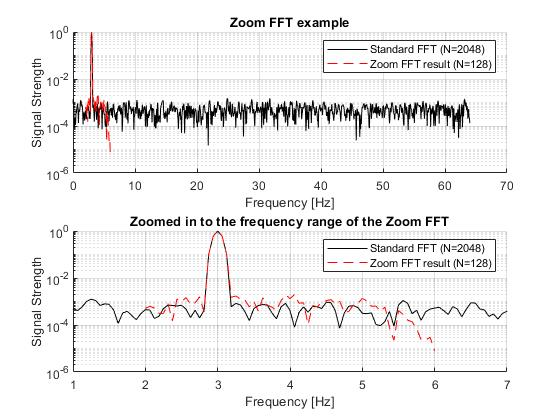
\includegraphics[scale=0.7]{MATLAB_zoom_fft_ex}
	\decoRule
	\caption{This figure shows the results of a Zoom FFT using the parameters listed in Table \ref{t:zoom_fft_parameters}.  The top plot shows the frequency spectrum from a standard FFT (black) and a Zoom FFT (red).  The bottom plot shows the same data as the top plot, but zoomed into a narrow frequency range. The standard FFT has a length of 2048, while the Zoom FFT has a length of 128.  This figure was created with MATLAB.}
	\label{fig:MATLAB_zoom_fft_ex}
\end{figure}

\subsubsection{Estimating processor performance}
Comparing the computational time of different algorithms is difficult because the dominant factor is usually memory access, rather than actual floating-point operations \cite{nussbaumer2012fast}.  Evaluating the computational cost due to memory access patterns in complicated, so this analysis will only consider the computational cost of the floating-point operations (FLOPs).  To minimize the cost from memory access patterns, the algorithms will be vectorized and converted to matrix form.  Most processors have highly optimized matrix operation functions, which should hopefully make arithmetic the dominant factor when determining the computational cost.

For this analysis, a STM32 processor is used as the baseline for estimating cycle counts because it is the unit used to prototype the LifeLine data acquisition device that collects experimental acceleration data from the turbine.  The STM32 has its own single precision register set to handle floating-point operations with hardware (rather than using compiled C libraries to perform the floating-point operations in many complex steps).  The floating-point unit (FPU) in the STM32 offers arithmetic instructions for the operations listed in Table \ref{t:stm32_cycles} \cite{stm32_floating_point}.

Many FPUs (like the one in Table \ref{t:stm32_cycles}), have multiply/accumulate arithmetic instructions, which means they can perform a multiplication and addition all in one step.  Additionally, division operations are much more expensive than multiplication operations and should be avoided as much as possible when designing algorithms.

Using the estimated floating point performance, the estimated clock cycles are shown in Table \ref{t:estimated_cycles}.  These are very rough estimates of the computational power required to perform each of the 3 FFT techniques.  The number of clock cycles for the FFT calculation is estimated from the Cooley Tukey algorithm \cite{puschel2007algebraic}.   The windowed FFT (shown in Figure \ref{fig:MATLAB_fft_window}) is not significantly more computationally expensive than a standard FFT, but performs much better.  The Zoom FFT analyzed in this table is the same design from Table \ref{t:zoom_fft_parameters} and Figure \ref{fig:MATLAB_zoom_fft_ex}.

\begin{table}[]
\centering
\caption{Cycle counts for a STM32 floating-point processor.  The exponential* operation is estimated from a floating-point performance analysis \cite{flops_performance} because it is not stated in the STM32 datasheet.}
\label{t:stm32_cycles}
\vspace*{0.2in}
\begin{tabular}{|c|c|}
\rowcolor[HTML]{EFEFEF} 
\hline
\textbf{Operation} & \textbf{Cycles} \\ \hline
Absolute value & 1 \\ \hline
Negate of a float & 1 \\ \hline
Addition/subtraction & 1 \\ \hline
Multiply & 3 \\ \hline
Multiply and accumulate/subtract & 3 \\ \hline
Divide & 14 \\ \hline
Square Root & 14 \\ \hline
Exponential & 20* \\ \hline
\end{tabular}
\end{table}

\begin{table}[]
\centering
\caption{Estimated cycle counts for various FFT techniques.}
\label{t:estimated_cycles}
\vspace*{0.2in}
\begin{tabular}{l|c|c|c|c|c|}
\cline{2-6}
                                                                    & \multicolumn{2}{c|}{\cellcolor[HTML]{C0C0C0}\textbf{\begin{tabular}[c]{@{}c@{}}Number of \\ Operations\end{tabular}}}                    & \multicolumn{3}{c|}{\cellcolor[HTML]{C0C0C0}\textbf{\begin{tabular}[c]{@{}c@{}}Number of Clock \\ Cycles {[}kCycles{]}\end{tabular}}} \\ \hline
\rowcolor[HTML]{C0C0C0} 
\multicolumn{1}{|l|}{\cellcolor[HTML]{C0C0C0}\textbf{Method}}       & \textbf{\begin{tabular}[c]{@{}c@{}}Multiply/\\ Accumulate\end{tabular}} & \textbf{\begin{tabular}[c]{@{}c@{}}FFT \\ Length\end{tabular}} & \textbf{Multiply}                             & \textbf{FFT}                             & \textbf{Total}                            \\ \hline
\multicolumn{1}{|l|}{\cellcolor[HTML]{C0C0C0}\textbf{Standard FFT}} & 0                                                                       & 1024                                                           & 0                                             & 435.2                                    & 435.2                                      \\ \hline
\multicolumn{1}{|l|}{\cellcolor[HTML]{C0C0C0}\textbf{Windowed FFT}} & 1024                                                                    & 1024                                                           & 3.072                                         & 435.2                                    & 438.3                                      \\ \hline
\multicolumn{1}{|l|}{\cellcolor[HTML]{C0C0C0}\textbf{Zoom FFT}}     & 512                                                                     & 128                                                            & 1.536                                         & 38.1                                     & 39.6                                       \\ \hline
\end{tabular}
\end{table}



\subsection{Goertzel Algorithm}
The Goertzel algorithm is a method for calculating individual bins of a discrete Fourier transform (DFT) without calculating all of the bins.  Since imbalance detection depends on the strength of the rotor frequency, this algorithm produces the particular rotor frequency bin value without calculating the entire DFT.  Fundamentally, this algorithm operates similarly to the Zoom FFT previously described, and is often called a Goertzel filter because the algorithm takes the form of a digital filter.  This algorithm applies 2 stages of filtering, where the first stage is an infinite impulse response (IIR) filter, and the second stage is a finite impulse response (FIR) filter.

For the first stage of the Goertzel algorithm, a 2nd order IIR filter is applied to $x$:
\begin{equation}
	s[n] = x[n] + 2 \cos{(\omega_0)}s[n-1] - s[n-2] \\
\end{equation}

This IIR filter follows a Direct Form II structure, where 2 state variables are required for a 2nd order filter.  $\omega_0$ is defined as the normalized frequency to be analyzed.

The second stage of the algorithm is a FIR filter, which is known for its linear phase, and lack of feedback.  This means that the filter output does not depends on any previous outputs.
\begin{equation} \label{eq:goertzel_output}
	y[n] = s[n] - e^{-j\omega_0}s[n-1]
\end{equation}

Equation \ref{eq:goertzel_output} shows the output of the Goertzel equation, $y[n]$.

There is an optimized version of the Goertzel algorithm that is even faster than the general form, but it produces squared magnitude components at each frequency instead of real/imaginary pairs \cite{embedded_goertzel}.  The phase of the frequency component is not used in the imbalance detection algorithm, so the optimized Goertzel algorithm is well suited for this application.  One of the benefits of the Goertzel algorithm is the buffer lengths do not need to be a power of 2.  An overview of the algorithm in a block diagram form is shown in Figure \ref{fig:goertzel_diagram_ti}.

The Goertzel algorithm is simulated with MATLAB and the results are shown in Figure \ref{fig:MATLAB_goertzel_algorithm_ex}.  The Goertzel algorithm calculates individual frequency components of the DFT, which are identical to the values calculated with a standard FFT algorithm.

\begin{figure}
	\centering
	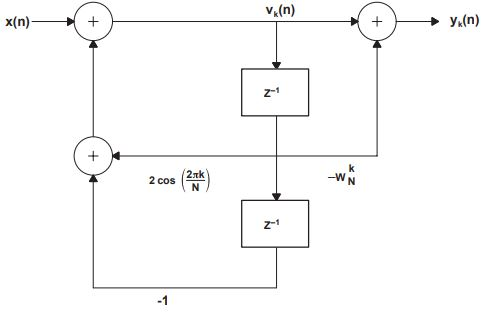
\includegraphics[scale=0.7]{goertzel_diagram_ti}
	\decoRule
	\caption{The direct-form realization of the Goertzel Algorithm\cite{TI_goertzel}.}
	\label{fig:goertzel_diagram_ti}
\end{figure}

\begin{figure}
	\centering
	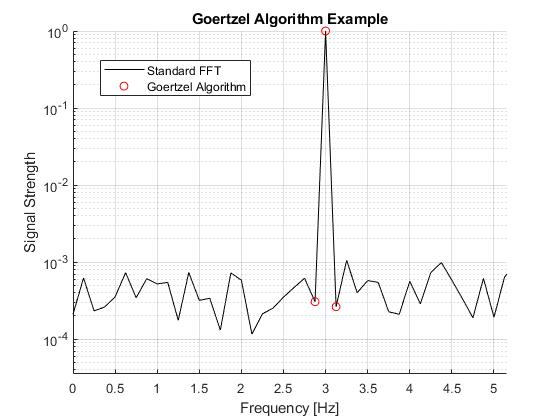
\includegraphics[scale=0.7]{MATLAB_goertzel_algorithm_ex}
	\decoRule
	\caption{This figure shows the frequency spectrum calculated with a standard FFT (black) and a few points calculated with the Goertzel algorithm (red).  This figure was created in MATLAB.}
	\label{fig:MATLAB_goertzel_algorithm_ex}
\end{figure}
